\documentclass[preprint, 3p, authoryear]{elsarticle} %review=doublespace preprint=single 5p=2 column
%%% Begin My package additions %%%%%%%%%%%%%%%%%%%

\usepackage[hyphens]{url}

  \journal{Transportation Research Part B: Methodological} % Sets Journal name

\usepackage{graphicx}
%%%%%%%%%%%%%%%% end my additions to header

\usepackage[T1]{fontenc}
\usepackage{lmodern}
\usepackage{amssymb,amsmath}
% TODO: Currently lineno needs to be loaded after amsmath because of conflict
% https://github.com/latex-lineno/lineno/issues/5
\usepackage{lineno} % add
\usepackage{ifxetex,ifluatex}
\usepackage{fixltx2e} % provides \textsubscript
% use upquote if available, for straight quotes in verbatim environments
\IfFileExists{upquote.sty}{\usepackage{upquote}}{}
\ifnum 0\ifxetex 1\fi\ifluatex 1\fi=0 % if pdftex
  \usepackage[utf8]{inputenc}
\else % if luatex or xelatex
  \usepackage{fontspec}
  \ifxetex
    \usepackage{xltxtra,xunicode}
  \fi
  \defaultfontfeatures{Mapping=tex-text,Scale=MatchLowercase}
  \newcommand{\euro}{€}
\fi
% use microtype if available
\IfFileExists{microtype.sty}{\usepackage{microtype}}{}
\usepackage[]{natbib}
\bibliographystyle{elsarticle-harv}

\ifxetex
  \usepackage[setpagesize=false, % page size defined by xetex
              unicode=false, % unicode breaks when used with xetex
              xetex]{hyperref}
\else
  \usepackage[unicode=true]{hyperref}
\fi
\hypersetup{breaklinks=true,
            bookmarks=true,
            pdfauthor={},
            pdftitle={Optimal departure time choices as quantiles and expectiles of the travel time distribution},
            colorlinks=false,
            urlcolor=blue,
            linkcolor=magenta,
            pdfborder={0 0 0}}

\setcounter{secnumdepth}{5}
% Pandoc toggle for numbering sections (defaults to be off)


% tightlist command for lists without linebreak
\providecommand{\tightlist}{%
  \setlength{\itemsep}{0pt}\setlength{\parskip}{0pt}}

% From pandoc table feature
\usepackage{longtable,booktabs,array}
\usepackage{calc} % for calculating minipage widths
% Correct order of tables after \paragraph or \subparagraph
\usepackage{etoolbox}
\makeatletter
\patchcmd\longtable{\par}{\if@noskipsec\mbox{}\fi\par}{}{}
\makeatother
% Allow footnotes in longtable head/foot
\IfFileExists{footnotehyper.sty}{\usepackage{footnotehyper}}{\usepackage{footnote}}
\makesavenoteenv{longtable}



\usepackage{booktabs}
\usepackage{longtable}
\usepackage{array}
\usepackage{multirow}
\usepackage{wrapfig}
\usepackage{float}
\usepackage{colortbl}
\usepackage{pdflscape}
\usepackage{tabu}
\usepackage{threeparttable}
\usepackage{threeparttablex}
\usepackage[normalem]{ulem}
\usepackage{makecell}
\usepackage{xcolor}



\usepackage{amsthm}
\newtheorem{theorem}{Theorem}[section]
\newtheorem{lemma}{Lemma}[section]
\newtheorem{corollary}{Corollary}[section]
\newtheorem{proposition}{Proposition}[section]
\newtheorem{conjecture}{Conjecture}[section]
\theoremstyle{definition}
\newtheorem{definition}{Definition}[section]
\theoremstyle{definition}
\newtheorem{example}{Example}[section]
\theoremstyle{definition}
\newtheorem{exercise}{Exercise}[section]
\theoremstyle{definition}
\newtheorem{hypothesis}{Hypothesis}[section]
\theoremstyle{remark}
\newtheorem*{remark}{Remark}
\newtheorem*{solution}{Solution}
\begin{document}


\begin{frontmatter}

  \title{Optimal departure time choices as quantiles and expectiles of the travel time distribution}
    \author[hwr]{Maria Osipenko%
  \corref{cor1}%
  }
   \ead{osipenko@hwr-berlin.de} 
      \affiliation[hwr]{
    organization={Hochschule für Wirtschaft und Recht Berlin},addressline={Badensche Str. 50},city={Berlin},postcode={10825},country={Germany},}
    \cortext[cor1]{Corresponding author}
  
  \begin{abstract}
  We consider two alternative preference specifications for optimal departure time choices: the classical asymmetric linear loss for early and late delays, and a new specification based on asymmetric quadratic loss. We demonstrate that the resulting optimal choices correspond to the tail indices of the travel time distribution---quantiles for the asymmetric linear specification and expectiles for the asymmetric quadratic specification. Additionally, we establish a correspondence between the choices induced by these two utility specifications, showing that the asymmetric quadratic preference class is a valid alternative with favorable properties, as demonstrated through examples and applications. For both utility specifications, we derive travel time reliability ratios and present a straightforward computation method using the concepts of \(\tau\)-deviation and \(\tau\)-variance. Moreover, we test both specifications using departure time choice data, finding that the quadratic loss specification more accurately represents actual departure time choices. Finally, using Montreal travel time data for two alternative routes, we fit a mixture of gamma distributions and compare the behavior of the optimal departure time choices and travel time reliability ratio curves induced by the different utility specifications.
  \end{abstract}
    \begin{keyword}
    scheduling utility \sep asymmetric loss \sep expectiles \sep quantiles \sep 
    travel time reliability
  \end{keyword}
  
 \end{frontmatter}

\hypertarget{background}{%
\section{Background}\label{background}}

Models of departure time choices often incorporate a scheduling component, where disutility or costs from early or late arrival, weighted by preference parameters, come into play. The majority of these models rely on an asymmetric linear scheduling component (\citet{fosgerau2010}, \citet{zhang2016}, \citet{guo2017}, \citet{li2019}, \citet{jin2020}). For example, \citet{fosgerau2010} specify the scheduling utility as:

\begin{equation}U_1(d,T) = -\{\alpha T + \beta(d-T)\mathbf 1_{T<d} + \gamma (T-d)\mathbf 1_{T\geq d}\}, \label{eq:u1}
\end{equation}

where \(T\) is a random travel time with cumulative distribution function \(F\), \(0<\beta<\alpha<\gamma\) are the preference parameters, the preferred arrival time is normalized to \(0\), and \(-d\), \(d>0\) is the departure time to choose.
\citet{fosgerau2010} demonstrate that the optimal departure time is equal to \(d_1^* = \mu + \sigma F^{-1}\left(\frac{\gamma}{\beta+\gamma}\right)\). This type of utility function assumes strictly increasing cumulative distribution function \(F\) of the travel time \(T\), such that the inverse \(F^{-1}\left(\frac{\gamma}{\beta+\gamma}\right)\) exists for all possible preference parametrizations \(\beta\) and \(\gamma\). Therefore, this scheduling approach may not be suitable for discrete travel time distributions or mixture distributions with a discrete component as in \citet{depalma2006}. In \citet{depalma2006}, the authors sensibly model the travel time distribution as a mixture of a continuous part on bad days and a discrete component on good days. For their analysis of risk preferences with information value, they employ classical mean-variance and mean-deviation utility functions, as well as other standard utilities with constant absolute and constant relative risk aversion. Later in the generalized setting, \citet{depalma2012} assume a differentiable utility function, which rules out the specification in \eqref{eq:u1}. However, the latter arguably describes the scheduling choice more authentically than the utility specifications in \citet{depalma2006}.

In this paper, we propose an alternative specification of the scheduling component. Specifically, we define:
\begin{equation}U_2(d,T) = -\{\alpha T + \beta(d-T)^2\mathbf 1_{T<d} + \gamma (T-d)^2\mathbf 1_{T\geq d}\}. \label{eq:u2}
\end{equation}
The above utility introduces an asymmetric \emph{quadratic} loss on early or late arrival. In this preference formulation, the marginal disutility \emph{increases linearly with the delay magnitude}, potentially describing the preferences of at least some commuters more consistently. Notably, this \emph{continuously differentiable} preference specification fulfills the assumptions of \citet{smith1984} and \citet{daganzo1985} required for the existence and uniqueness of equilibrium in a single bottleneck model. It also satisfies the requirements of \citet{depalma2012} and their equilibrium analysis under risk aversion and information value.

Both preference specifications in \eqref{eq:u1} and \eqref{eq:u2} share the property that the optimal departure time choices correspond to specific \emph{tail indices} of the travel time distribution. For the first specification in \eqref{eq:u1}, these are the \emph{quantiles}, and for the second specification in \eqref{eq:u2}, these are the \emph{expectiles} of the travel time. The asymmetric quadratic version of the scheduling preferences, and the fact that the solutions to the expected utility maximization problem are quantiles and expectiles (and in general the so-called \(L_p\)-quantiles) as \emph{the minimizers of expectations in asymmetric} \(L_p\)\emph{-norms}, seem to have been largely unaddressed explicitly in the previous literature. Moreover, both types of the scheduling preferences are related via the quantile-expectile correspondence (\citet{jones1994}), with the second version in \eqref{eq:u2} describing a class of preferences with more favorable properties to the first, as demonstrated below.

In this paper, we analyse and compare the two utility specifications of scheduling preferences: the linear one in \eqref{eq:u1} and the quadratic one in \eqref{eq:u2}, with the latter offering advantages over the former. First, we review the existing specification and formally define the new asymmetric quadratic utility in Section 2. In Section 3, we introduce the concepts of quantiles and expectiles as the minimizers of expectations in the respective asymmetric \(L_p\)-norms, and show that the optimal departure times are the quantiles of \(T\) for the linear (\(p=1\)) and the expectiles of \(T\) for the quadratic (\(p=2\)) case. Furthermore, we link the optimal choices derived from the two utility specifications through the concept of quantile-expectile correspondence and demonstrate that the new asymmetric quadratic class is valid alternative, offering conceptional and computational advantages over the linear asymmetric case in \eqref{eq:u1}. We also derive the travel time reliability ratios to quantify travel time reliability for both utility specifications and propose their estimation using the related concepts of \(\tau\)-deviation and \(\tau\)-variance to complete Section 3. Using Montreal travel time data, we compare in Section 4 the optimal departure time choices for two routes and the resulting travel time reliability ratios based on a fitted mixture of gamma distributions with two components representing the free-flow and congestion regimes. Finally, we conclude and discuss the implications.

\hypertarget{asymmetric-scheduling-preferences}{%
\section{Asymmetric scheduling preferences}\label{asymmetric-scheduling-preferences}}

Consider a traveler with a utility function depending on random travel time \(T\) with realizations \(t\in\mathbb R_+\) and on departure time \(-d\) for \(d>0,\) with the preferred arrival time normalized to \(0\). Assume the following utility function for the traveler, where \(\alpha,\beta, \gamma>0\) are preference parameters underlying the relative importance of total travel time, early and late delays respectively:

\begin{align}
U_a(d,T) = -\{\alpha T + \beta(d-T)^a\mathbf 1_{T<d} + \gamma (T-d)^a\mathbf 1_{T\geq d}\}, ~~a\in\{1,2\}.\label{eq:ua}
\end{align}

For \(a=1\) in \eqref{eq:ua}, we recover the scheduling approach of \citet{fosgerau2010} and arrive at the utility function already specified in \eqref{eq:u1}:

\[U_1(d,T) = -\{\alpha T + \beta(d-T)\mathbf 1_{T<d} + \gamma (T-d)\mathbf 1_{T\geq d}\}.\]

As in \citet{small1982} and \citet{small2015}, we require \(\gamma>\beta>0\). In this formulation, both early and late arrivals increase the disutility of the traveler in a \textbf{linear} manner, with the marginal disutility of early arrival being equal to \(\beta\) and the marginal disutility of late arrival being equal to \(\gamma\). Note that the utility decrease is asymmetric regarding the type of delay (early or late).

The asymmetric linear loss may be unrealistic in many situations, as the marginal disutility of early or late delays is constant and does not depend on the magnitude of the delay. For instance, \citet{enide2006} find that extremely long travel times influence significantly the route choice. \citet{vanlint_etal08} advocate approaches to travel time reliability measurement that account for extreme travel times. \citet{sikka_hanley13} find that commuters exhibit high sensitivities towards unreliable routes, on which extremely long travel times are possible. When the marginal disutility increases along with the delay magnitude, asymmetric \textbf{quadratic} loss describes such preferences in a way, more consistent with the empirical findings above. In fact, such a specification of the traveler utility function even simplifies the computation of the optimal departure time, as we show later. The asymmetric quadratic version of \(U_a(d,T)\) in \eqref{eq:ua} with \(a=2\), mentioned previously in \eqref{eq:u2}, reads:

\[U_2(d,T) = -\{\alpha T + \beta(d-T)^2\mathbf 1_{T<d} + \gamma (T-d)^2\mathbf 1_{T\geq d}\}.\]

The marginal disutility of an early arrival (\(d>t\)) becomes \(\beta (d-t)\) and the marginal disutility of a late arrival (\(d\leq t\)) becomes \(\gamma (t-d)\). The above formulation of preferences has the advantage of being differentiable with respect to \(d\), which is a necessary condition for the uniqueness of the resulting equilibrium distribution of arrivals in a single bottleneck model (\citet{daganzo1985}). Moreover, both utility functions are reformulations of cost functions in departure time choice problems in single bottlenecks as specified by \citet{lindsey2004}.

We assume that the traveler maximizes her expected utility \(\big(\mathbb E(\cdot)\) denotes the expectation with respect to the distribution of \(T\) \(\big)\), which corresponds:

\begin{itemize}
\item
  \textbf{linear asymmetric case}:
  \begin{equation}\mathbb EU_1(d,T) = -\left[\alpha \mathbb ET + \beta\mathbb E\left\{(d-T)\mathbf 1_{T<d} \right\}+ \gamma \mathbb E\left\{(T-d)\mathbf 1_{T\geq d}\right\}\right], \label{eq:eu1}
  \end{equation}
\item
  \textbf{quadratic asymmetric case}:
  \begin{equation}
  \mathbb EU_2(d,T) = -\left[\alpha \mathbb ET + \beta\mathbb E\left\{(d-T)^2\mathbf 1_{T<d} \right\}+ \gamma \mathbb E\left\{(T-d)^2\mathbf 1_{T\geq d}\right\}\right]. \label{eq:eu2}
  \end{equation}
\end{itemize}

Both utility formulations fall under the mean-dispersion framework (\citet{engelson2016}) with different notions of dispersion used. For \(\beta=\gamma\), \eqref{eq:eu1} corresponds to a symmetric mean-absolute deviation utility, and the optimal choice \(d^*_1\) corresponds to the median of the travel times. For \(\gamma>\beta\) it remains asymmetric, and the second term in the maximized expected utility \(\mathbb EU^*_1(d_1^*,T)\) is an asymmetric version of the absolute deviation, termed in \citet{tran2019} as the \textbf{\(\tau\)-deviation} (asymmetrically weighted absolute deviation around the \textbf{\(\tau\)-quantile}). Similarly, for \(\beta=\gamma\), \eqref{eq:eu2} becomes \(\mathbb EU_2(d,T) = -\left[\alpha \mathbb ET + \beta\mathbb E\left\{(T-d)^2\right\}\right]\),
which is maximized for \(d_2^* = \mathbb ET\). Hence, we recover the classical mean-variance utility \(\mathbb EU^*_2(d_2^*,T)\) used by \citet{jackson1982}. For \(\gamma>\beta\) the second term in the maximized expected utility \(\mathbb EU^*_2(d_2^*,T)\) is a generalized version of the variance - \textbf{the \(\tau\)-variance} - around a certain tail index - \textbf{the \(\tau\)-expectile}.

\hypertarget{optimal-departure-time-choice-under-asymmetric-scheduling-preferences}{%
\section{Optimal departure time choice under asymmetric scheduling preferences}\label{optimal-departure-time-choice-under-asymmetric-scheduling-preferences}}

In this section, we demonstrate that the optimal departure time is equal to a certain quantile (see \citet{koenker1978}) in case of \(U_1(d,T)\) and a certain expectile (see \citet{newey1987}) for \(U_2(d,T)\) of the travel time distribution. The specific quantile or expectile levels depend on the asymmetry parameters (\(\beta\) and \(\gamma\)) of the traveler's utility function. Therefore, we briefly review the concepts of quantiles and expectiles in the following.

\hypertarget{quantiles-and-expectiles}{%
\subsection{Quantiles and expectiles}\label{quantiles-and-expectiles}}

Quantiles and expectiles are real numbers that describe the distribution of a real random variable \(X\). They generalize the median and the mean, respectively, to their asymmetric versions via the asymmetry index \(\tau\in(0,1)\). For a suitable set of such indices \(\tau\in(0,1)\), the associated sets of either quantiles \(\{q_\tau(X)\}_{\tau\in(0,1)}\) or expectiles \(\{e_\tau(X)\}_{\tau\in(0,1)}\) are capable of representing the entire distribution of a random variable.

Both quantiles and expectiles can be viewed as minimizers of the expectations of the corresponding asymmetric norms (see e.g. \citet{tran2019}):
\begin{align}
\min_{c\in\mathbb R}\mathbb E_{F_X}||X-c||^a_{a,\tau}, \text{ for } a\in\{1,2\}, \label{eq:asnorm}
\end{align}
where \(||x||^a_{a,\tau}=|x|^a\cdot\{\tau\mathbf 1_{x\geq 0}+(1-\tau)\mathbf 1_{x<0}\}\) is the \(\ell_a\) asymmetric norm for \(x\in\mathbb R\).
That is, the \(\tau\)-quantile solves:
\begin{equation}q_\tau(X) = \arg\min_{q\in\mathbb R}\mathbb E_{F_X}||X-q||^1_{1,\tau},\label{eq:quantile}
\end{equation}

whereas the \(\tau\)-expectile solves:
\begin{equation}
e_\tau(X) = \arg\min_{e\in\mathbb R}\mathbb E_{F_X}||X-e||^2_{2,\tau}.\label{eq:expectile}
\end{equation}
Unlike quantiles which only rely on frequencies, expectiles take into consideration both the frequency of extreme observations and their magnitude.
Moreover, expectiles are uniquely defined for random variables with finite first moments. For quantiles to be unique, a strictly increasing cumulative distribution function is required. For a non-decreasing cumulative distribution function, the quantile function can be defined as \(q_\tau(X) = \inf\{x\in \mathbb R: \tau\leq F(x)\}\), which is well-defined. Nevertheless, as shown in the next chapter, all values \(\{x\in\mathbb R: \tau= F(x)\}\) induce the same expected scheduling utility level as maximizers of \eqref{eq:eu1} and result in ambiguous choices. The latter fact can create difficulties in treating, for instance, discrete distributions as the examples below show.

\hypertarget{quantiles-and-expectiles-for-different-travel-time-models}{%
\subsubsection{Quantiles and expectiles for different travel time models}\label{quantiles-and-expectiles-for-different-travel-time-models}}

Since we are concerned with modelling departure time choice within the framework of quantiles and expectiles, we provide several examples that align with the models of travel time distribution proposed in the literature.

\begin{example}[Quantiles and expectiles of a two-value travel time distribution]
\protect\hypertarget{exm:ddqande}{}\label{exm:ddqande}In this example, we consider a discrete two-value travel time distribution. \citet{depalma2006} use this type of distribution to model travel times on an uncertain route in their analysis. Another example is an ideal road link without congestion, where two speed regimes might exist depending on whether the road surface is wet or not (or whether there is fog or not). In this case, \(1-p\) could represent the probability of a wet surface or the probability of rain. Yet another scenario where such a two-value discrete distribution may be applicable is bike-sharing. If a commuter uses a bike-sharing station within a short walking distance and finds no bikes available (with probability \(1-p\)), they would need to account for a longer travel time. Assuming there are no other traffic obstructions, walking and riding a bike at the same speed would result in just two possible travel times, depending on the walking distance in this case.

Consider random travel time \(T\) with two values: \(t_1\) with probability \(p\) and \(t_2\), such that \(t_2-t_1>0\), with probability \(1-p\).The resulting distribution of the travel time is presented in the left panel of Figure \ref{fig:figex1}.
For any \(\tau\in [0,p)\) the \(\tau\)-quantile corresponds to \(t_1\); likewise, for \(\tau\in (p,1]\) the \(\tau\)-quantile corresponds to \(t_2\). For \(\tau=p\), \(\mathbb P(T\leq t) = p\) for \(t\in[t_1,t_2)\) resulting in a non-unique \(\tau\)-quantile taking on any value in the range \([t_1,t_2)\). Following the classical definition of the quantile function in \citet{xiao12}, where the infimum among the possible values is taken to serve as the unique \(\tau\)-quantile:

\begin{equation}q_\tau(X) = \inf\{x\in \mathbb R: \tau\leq F(x)\},\label{eq:inf}
\end{equation}

we arrive at \(q_p = t_1\).

In case of the expectiles, using formulas (18) and (19) in \citet{holzmann2016} we have (in the following, we use the notation \(e_\tau\) for \(e_\tau(X)\) and \(q_\tau\) for \(q_\tau(X)\)):

\[e_\tau = \frac{(1-\tau)t_1p+ \tau t_2(1-p)}{(1-\tau)p + \tau(1-p)}.\]

This expression is continuous and strictly increasing in \(\tau\) (see Figure \ref{fig:figex1}).

\begin{figure}
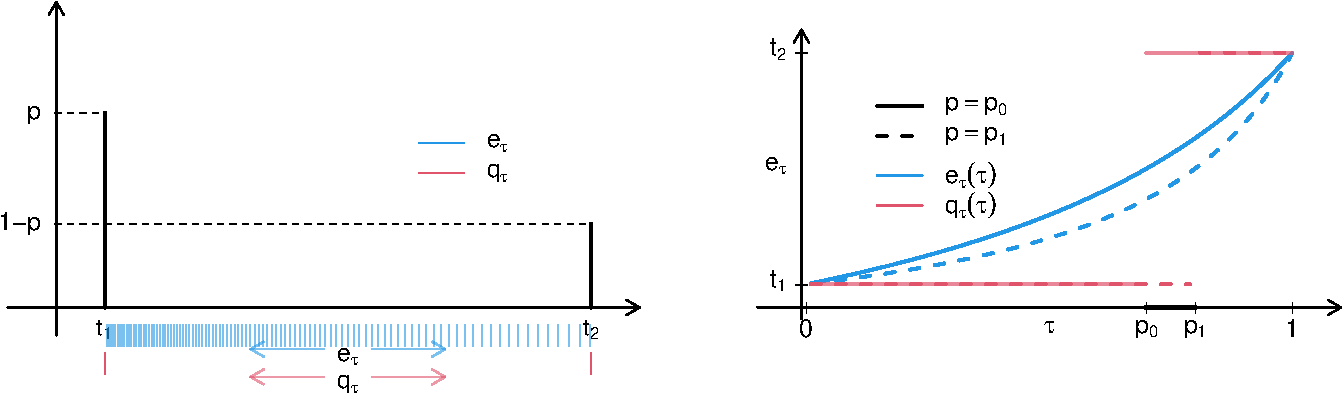
\includegraphics[width=1\linewidth]{traffic-expectiles_files/figure-latex/figex1-1} \caption{Right panel: the considered two-value travel time distribution and the expectile and quantile values (below the $x$-axis) in Example 3.1 for a grid of $\tau$-values. Left panel: the expectile and the quantile functions for the two-value discrete distribution with varying $p$. }\label{fig:figex1}
\end{figure}

Since \(\frac{\partial e_\tau}{\partial p} =(t_1-t_2)\cdot \frac{ \tau (1-\tau)} {\{\tau+p (1-2\tau )\}^2} <0,\) \(e_\tau\) decreases in \(p\) or, equivalently, it increases in \(1-p\). Note that increasing \(p\) from \(p_0\) to \(p_1\) affects only a small portion of quantiles (with indices \(\tau\in[p_0,p_1]\)), whereas it impacts all expectiles, as illustrated in the right panel of Figure \ref{fig:figex1}. The expression \(\frac{\partial e_\tau}{\partial t_2} =\frac{\tau (1-p)}{(1-\tau)p + \tau(1-p)} >0\) also reveals the impact of increasingly extreme travel times on all expectiles, regardless of the level \(\tau\). At the same time, only the upper quantiles for \(\tau>p\) are affected.

In summary, expectiles are more sensitive than quantiles to changes in the tail regions of the travel time distribution, making them useful for capturing sensitivity to extremes reported by \citet{enide2006}, \citet{vanlint_etal08}, and \citet{sikka_hanley13} in empirical analyses.
\end{example}

In the example above, we derive an explicit expression for \(e_\tau\). However, this is not always possible, and \(e_\tau\) is represented in an implicit functional form based on the first order condition of \eqref{eq:asnorm} for \(a=2\):

\begin{align}
\tau\mathbb E\{|Y-e_\tau|\mathbf 1_{Y>e_\tau}\} = (1-\tau)\mathbb E\{|Y-e_\tau|\mathbf 1_{Y\leq e_\tau}\}.\label{eq:etau}
\end{align}

Moreover, as \(e_\tau\) is continuous, strictly increasing in \(\tau\), and unique for each \(\tau\in(0,1)\) for all distributions \(F\) with finite expectation (\citet{holzmann2016}), there exist an inverse expectile function \(\tau(e_\tau)\). This function frequently does have an explicit functional form, making it convenient for analysis. In fact, the inverse expectile function is itself a cumulative distribution function with a density, but it generally differs from the original \(F\), as noted by \citet{philipps2022}.

Rearranging \eqref{eq:etau}, we get the following expression for the inverse expectile function:

\begin{align}
\tau(e_\tau) &= \frac{\mathbb E\{|Y-e_\tau|\mathbf 1_{Y\leq e_\tau}\}} {\mathbb E\{|Y-e_\tau|\}} = \frac{\mathbb E\{(Y-e_\tau)\mathbf 1_{Y\leq e_\tau}\}}{2\mathbb E\{(Y-e_\tau)\mathbf 1_{Y\leq e_\tau}\} - \mathbb E\{(Y-e_\tau)\}}. \label{eq:tau}
\end{align}

Below we provide another example with continuously distributed travel times, where \eqref{eq:tau} provides closed-form expression for the inverse expectile function.

\begin{example}[Quantiles and expectiles of a mixture of two uniform distribution with disjoint supports]
\protect\hypertarget{exm:duqande}{}\label{exm:duqande}Consider a random travel time \(T\) that follows a mixture of uniform distributions with ranges \([a_1,a_2]\) and \([a_3,a_4]\), respectively, and with mixing probability \(p\). We assume that \(a_1<a_2<a_3<a_4\), creating a ``gap'' in the support of the mixture distribution. For instance, we might consider a road link without congestion that operates under two speed regimes depending on an exogenous event \(I\), which takes values \({0,1}\) with probabilities \(p\) and \(1-p\), respectively. In the context of park-and-ride, this type of travel time distribution could arise due to a specific public service schedule and the resulting waiting time if commuters have to take a later service because of traffic congestion.

Let \(F\) denote the cumulative distribution function of \(T\). The quantile function for \(\tau <p\) is given by:
\[q_\tau = a_1 + \frac{a_2-a_1} p\tau.\]

For \(p<\tau\), it is given by:
\[q_\tau = a_3 + \frac{a_4-a_3}{1-p}(\tau-p).\]
However, when \(\tau=p\), any value in the range \((a_2,a_3)\) is a valid \(p\)-quantile. Using \eqref{eq:inf}, we get \(q_p=a_2\).

Starting with \eqref{eq:tau}, we compute the inverse expectile function \(\tau(e_\tau)\) as follows:

\[
\tau(e_\tau)=\begin{cases}
0, &e_\tau<a_1\\
\frac{-\frac 12 \frac{p}{a_2-a_1}(a_1-e_\tau)^2}{-\frac{p}{a_2-a_1}(a_1-e_\tau)^2    -\frac 12(p(a_1+a_2) + (1-p)(a_3+a_4)) + e_\tau}, & a_1\leq e_\tau<a_2,\\
\frac{\frac 12p\left(a_1 + a_2 - 2e_\tau\right)}{p\left(a_1 + a_2 - 2e_\tau\right)  -\frac 12(p(a_1+a_2) + (1-p)(a_3+a_4)) + e_\tau}, & a_2\leq e_\tau<a_3,\\
\frac{\frac 12 p\left(a_1 + a_2 - 2e_\tau\right)-\frac 12 \frac{1-p}{a_4-a_3}(a_3-e_\tau)^2}{p\left(a_1 + a_2 - 2e_\tau\right)-\frac{1-p}{a_4-a_3}(a_3-e_\tau)^2   -\frac 12(p(a_1+a_2) + (1-p)(a_3+a_4)) + e_\tau}, & a_3\leq e_\tau<a_4,\\
1, &e_\tau\geq a_4.
\end{cases}\]

The resulting expectile functions as functions of \(\tau\) for different \(p\) are presented in Figure \ref{fig:figexp1}.

\begin{figure}
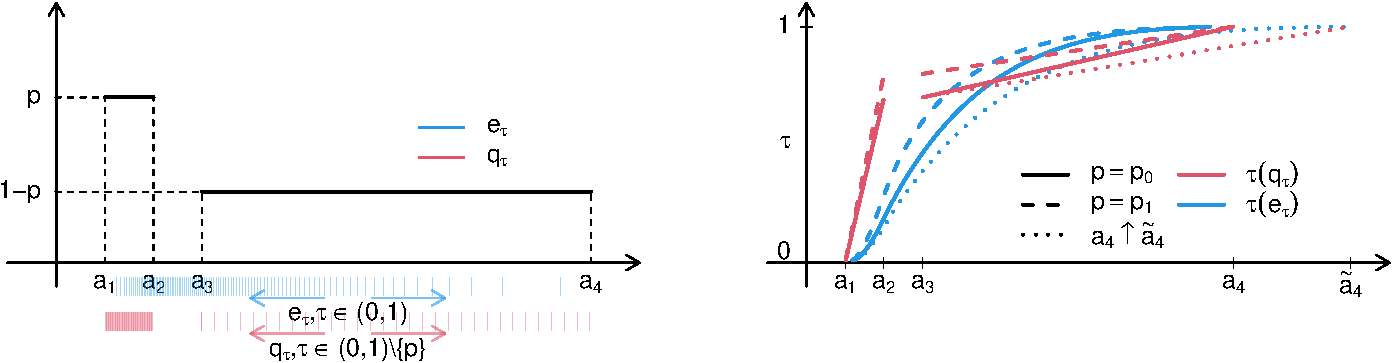
\includegraphics[width=1\linewidth]{traffic-expectiles_files/figure-latex/figexp1-1} \caption{Left panel: The considered mixture of two uniform distributions in Example 3.2 and the expectile and quantile values (below the $x$-axis) for a grid of $\tau$-values. Right panel: The inverse quantile and expectile functions for different mixing parameter $p$ and varying right extreme value $a_4$ in Example 3.2.}\label{fig:figexp1}
\end{figure}

Note that in this case, all expectiles and quantiles change with \(p\) (see the right panel of Figure \ref{fig:figexp1}). But what happens if we increase \(a_4\) to extend the extreme right end of the travel time? As in the previous example, all expectiles are affected, but only the upper quantiles (\(\tau>p\)) change.

In general, for mixtures of \(m\) disjoint (sorted) uniforms holds with mixing parameter vector \(\mathbf p=(p_1,\ldots,p_m)^\top\) where \(p_m=1-\sum_{i=1}^{m-1}p_i\) and support edges \(a_1<a_2<\ldots<a_{m+1}\):

\[\tau(e_\tau) = 
\begin{cases}
0,&e_\tau<a_1,\\
\frac{-\frac 12\frac{p_1}{a_2-a_1}(a_1-e_\tau)^2}  {-\frac{p_1}{a_2-a_1}(a_1-e_\tau)^2- \sum_{j=1}^mp_j\frac{a_{j+1}+a_j}2 +e_\tau} ,&a_1\leq e_\tau< a_2,\\
\frac{\frac 12\sum_{k=1}^{i-1}p_k\cdot (a_{k+1}+a_{k}-2e_\tau) -\frac 12 \cdot \frac{p_i}{a_{i+1}-a_i}(a_i-e_\tau)^2}  {\sum_{k=1}^{i-1}p_k\cdot (a_{k+1}+a_{k}-2e_\tau) -\frac{p_i}{a_{i+1}-a_i}(a_i-e_\tau)^2- \sum_{j=1}^mp_j\frac{a_{j+1}+a_j}2 +e_\tau} ,&a_i\leq e_\tau< a_{i+1},i=2,\ldots, m\\
1, &e_\tau\geq a_{m+1}.
\end{cases}\]
\end{example}

In Example \ref{exm:duqande}, we used a mixture of two continuous distributions to model travel time \(T\). However, mixture models with both discrete and continuous components were considered in the literature as well. For instance, to model urban arterial roads, \citet{zheng_fangfang2017} distinguish two regimes: undersaturated and oversaturated conditions. Under oversaturated conditions, the authors model the probability function of a delay as a mixture of several box shaped functions with bounded supports, which may not overlap as in Example \ref{exm:duqande}. The overall delay distribution in \citet{zheng_fangfang2017} is composed of a mixture of Dirac delta functions on a fixed free-flow time and several uniform delay distributions with bounded supports representing the effects of traffic lights, traffic control or similar conditions. As mentioned in \citet{zheng_fangfang2017}, the point mass at \(a_0\) can be substituted by a distribution centered at \(a_0\), since different vehicle or driver types may exhibit slightly varying free-flow times.

Within our framework, one can use a mixture of any appropriate distributions instead of the uniform mixture components. For instance, \citet{jabari2019} use mixture of gamma distributions for travel time modelling. In this case, \(\tau(e_\tau)\) has no closed-form expression; however, numeric computation based on Equation \eqref{eq:tau} is still feasible (see \citet{daouia_etal24}). For a given distribution, quantiles and expectiles can be obtained by Monte-Carlo approximation, where the sample counterparts, \(\hat q_\tau(X)\) and \(\hat e_\tau(X)\), of the population \(\tau\)-quantile (defined in \eqref{eq:quantile}) and \(\tau\)-expectile (defined in \eqref{eq:expectile}) are computed as plug-in estimators based on the empirical distribution function:

\begin{align}
\hat q_\tau(X) = \arg\min_{q\in\mathbb R}\sum_{i=1}^n||x_i-q||^1_{1,\tau}, \label{eq:q}
\end{align}
and

\begin{align}
\hat e_\tau(X) = \arg\min_{e\in\mathbb R}\sum_{i=1}^n||x_i-e||^2_{2,\tau}. \label{eq:e}
\end{align}

In this formulation, both are asymmetric versions of \emph{M-estimators} and \emph{M-quantiles} with the corresponding properties as consistency and, under some more restrictive assumptions as finite second moment and continuous \(F\), asymptotic normality (\citet{holzmann2016}, \citet{abdous1995}, \citet{breckling1988}). Moreover, as \citet{abdous1995} note, sample expectile estimators are \emph{more efficient} than sample quantiles.

In the following, we consider another example, where a mixture of gamma distributions id used to model travel time.

\begin{example}[Quantiles and expectiles of travel time distribution with continuous gamma components]
\protect\hypertarget{exm:qdzheng}{}\label{exm:qdzheng}Consider now a travel time distribution where there is a certain probability \(0<p_0<1\) that the free-flow travel time follows a gamma distribution with parameters \(k_f>0\) (shape) and \(\theta_f>0\) (scale) is attained. At the same time, congestion conditions occur with probability \(p\), and the travel time distribution under congestion is represented by another gamma distribution with higher mean and variance, parametrized by \(k_d>0\) and \(\theta_d>0\), such that \(k_f\theta_f<k_d\theta_d\) and \(k_f\theta^2_f<k_d\theta^2_d\).

To illustrate, we set \(k_f=10\), \(\theta_f=0.5\), \(k_c=20\), \(\theta_c=2\). This corresponds to a free-flow mean travel time of \(5\) minutes with a standard deviation of \(\approx 1.58\) minutes, and a mean congestion travel time of \(10\) minutes with a standard deviation of \(\approx 8.94\) minutes. The quantiles and expectiles are obtained by Monte-Carlo approximation (\citet{daouia_etal24}).

\begin{figure}
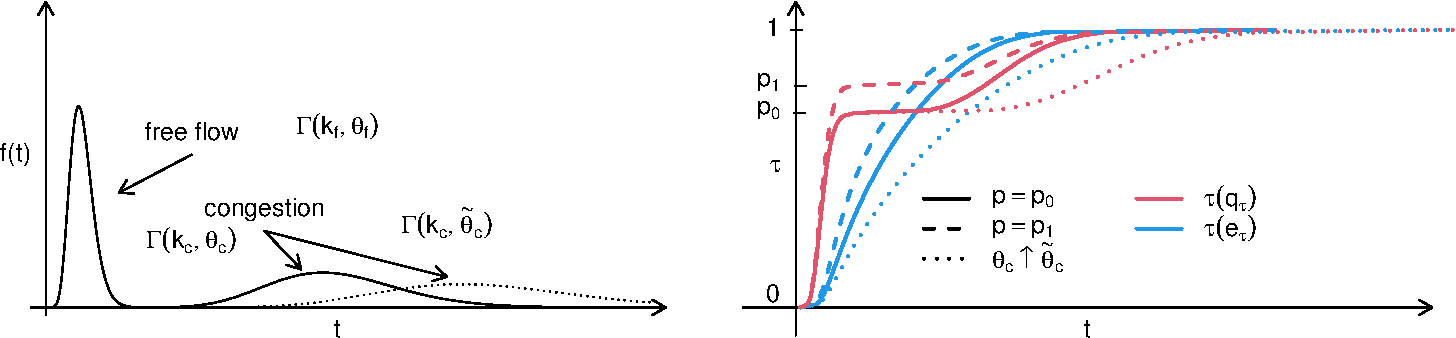
\includegraphics[width=1\linewidth]{traffic-expectiles_files/figure-latex/figexp3-1} \caption{Left panel: The considered mixture of two gamma distributions in Example 3.3. Right panel: The inverse quantile and expectile functions for different parameter values for $p$ and $  heta$ in Example 3.3.}\label{fig:figexp3}
\end{figure}

In this example, the mixture distribution has a continuous density, and both the (inverse) quantile and the expectile functions are smooth. Nevertheless, in low probability regions, the quantile function is rather ``flat'', exhibiting a drastic change in value for a small change in \(\tau\). As in the previous example, we observe similar effects resulting from changing the mixture parameter \(p\) and extending the right tail probability of the congestion state (by increasing the scale \(\theta\)). Only the upper quantiles (\(\tau>p\)) respond to changes in the congestion distribution; there is a clear distinction between the effects of changing \(p\) the upper (high impact) and lower quantiles (low impact). In contrast, the effects on the expectiles are more evenly distributed.
\end{example}

\hypertarget{properties-of-quantiles-and-expectiles}{%
\subsubsection{Properties of quantiles and expectiles}\label{properties-of-quantiles-and-expectiles}}

Being quantile-alike tail indices, expectiles share some properties of quantiles, such as location and scale equivariance. To be able to compare both tail indices later in the analysis, we provide their important properties below. Moreover, there exists a correspondence between quantiles and expectiles, which allows to interchange their use. We summarize the properties in the upcoming propositions.

\begin{proposition}[Location and scale equivariance of quantiles and expectiles]
\protect\hypertarget{prp:propprops}{}\label{prp:propprops}

Let \(Y\in\mathbb R\) be a random variable with finite expectation; then, for \(\tau \in (0,1)\) and \(s>0\):

\begin{itemize}
\item
  \(q_\tau(sY+m) = sq_\tau(Y) + m\) (follows from location and scale equivariance of the quantile loss function) and
\item
  \(e_\tau(sY+m)=se_\tau(Y) + m\) (Theorem 1 in \citet{newey1987}).
\end{itemize}

\end{proposition}

The properties above are useful for analysing the role of the mean and the variance of travel time distribution for optimal departure time plans.

Another useful property is the existence of the correspondence between (well-defined) quantiles and expectiles (see \citet{jones1994}, \citet{yao1996} and \citet{waltrup2015}) of a distribution.

\begin{proposition}[Quantile-expectile correspondence]
\protect\hypertarget{prp:corr}{}\label{prp:corr}For each well-defined \(\tau_1\)-quantile, there exists \(\tau_2(\tau_1)\in(0,1)\) such that \(q_{\tau_1}(Y) = e_{\tau_2(\tau_1)}(Y).\)
The correspondence function between quantiles and expectiles of a random Variable \(T\in \mathbb R\) with distribution function \(F\), \(\tau_2(\tau_1):(0,1)\rightarrow(0,1)\) is given by:
\[\tau_2 (\tau_1) = \frac{-q_{\tau_1}\tau_1 + G(q_{\tau_1})}{-\mathbb EY + 2G(q_{\tau_1})+q_{\tau_1}(1-2\tau_1)},\]
where \(G(q) = \int_{-\infty}^qt~dF(t)\) is the partial moment function.
\end{proposition}

\begin{proof}
The proof follows \citet{yao1996} who proof the result in a regression context.

For any distribution \(F\) with finite mean, the expectile function \(\tau_2\rightarrow e_{\tau_2}(F)\) is continuos, strictly increasing and has range \(\{y\in\mathbb R: 0<F(y)<1\}\). So, for each well defined quantile \(q_{\tau_1}=F^{-1}(\tau_1)\) there exists \(\tau_2\) such that:
\[q_{\tau_1}(F) = e_{\tau_2}(F).\]

Following \citet{yao1996} and using the following identity for \(\tau_2\):
\[\tau_2 = \frac{\mathbb E(|Y-e_{\tau_2}|\mathbf 1_{Y\leq e_{\tau_2}})}{\mathbb E(|Y-e_{\tau_2}|\mathbf 1_{Y\leq e_{\tau_2}}) + \mathbb E(|Y-e_{\tau_2}|\mathbf 1_{Y> e_{\tau_2}})},\]

we get:
\begin{align*}\tau_2 (\tau_1) &= \frac{\mathbb E(|Y-q_{\tau_1}|\mathbf 1_{Y\leq q_{\tau_1}})}{\mathbb E(|Y-q_{\tau_1}|\mathbf 1_{Y\leq q_{\tau_1}}) + \mathbb E(|Y-q_{\tau_1}|\mathbf 1_{Y> q_{\tau_1}})},\\
&= \frac{-\mathbb E(Y\mathbf 1_{Y\leq q_{\tau_1}})+q_{\tau_1}\tau_1}{\mathbb E(Y\mathbf 1_{Y\leq q_{\tau_1}})-q_{\tau_1}\tau_1 + \mathbb E(Y\mathbf 1_{Y> q_{\tau_1}})-q_{\tau_1}(1-\tau_1)},\\
&= \frac{-\mathbb E(Y\mathbf 1_{Y\leq q_{\tau_1}})+q_{\tau_1}\tau_1}{\mathbb EY - 2\mathbb E(Y\mathbf 1_{Y\leq q_{\tau_1}})-q_{\tau_1}(1-2\tau_1)}.
\end{align*}

Rewriting \(\mathbb E(Y\mathbf 1_{Y\leq q}) = G(q)\), we obtain:

\[\tau_2 (\tau_1) = \frac{-q_{\tau_1}\tau_1 + G(q_{\tau_1})}{-\mathbb EY + 2G(q_{\tau_1})+q_{\tau_1}(1-2\tau_1)}.\]
\end{proof}

Using the above correspondence between quantiles and expectiles, a comparison of the optimal plans for the two parameterizations of the utility function is straightforward.

\begin{example}[Correspondence between quantiles and expectiles]
\protect\hypertarget{exm:corrqe}{}\label{exm:corrqe}Consider \(T\) with the uniform mixture distribution as in Example \ref{exm:duqande}. The correspondence function between the associated \(\omega\)-quantile and the \(\tau\)-expectile of \(T\) \(\tau(\omega):(0,1)\setminus\{0.7\}\rightarrow(0,1)\) is given by:

\[\tau(\omega)=\begin{cases}
\frac{-\omega q_\omega+ \frac 12 \frac p{a_2-a_1}(q_\omega^2-a_1^2)}{-\frac{p(a_1+a_2)}{2}-\frac{(1-p)(a_3+a_4)}{2} +\frac p{a_2-a_1}(q_\omega^2-a_1^2) + (1-2\omega)q_\omega},&q_\omega= a_1 + \frac{a_2-a_1} p\omega, \omega <p\\
\frac{-\omega q_\omega(T) + \frac 12 p(a_1+a_2) + \frac 12 \frac {1-p}{a_4-a_3}(q_\omega^2-a_3^2)}{-\frac{(1-p)(a_3+a_4)}{2} + \frac{p(a_1+a_2)}2 + \frac {1-p}{a_4-a_3}(q^2-a_3^2) + (1-2\omega)q_\omega},&q_\omega = a_3 + \frac{a_4-a_3}{1-p}(\omega-p), p<\omega
\end{cases}\]

and is shown in Figure \ref{fig:figcor}.
\end{example}

\begin{figure}
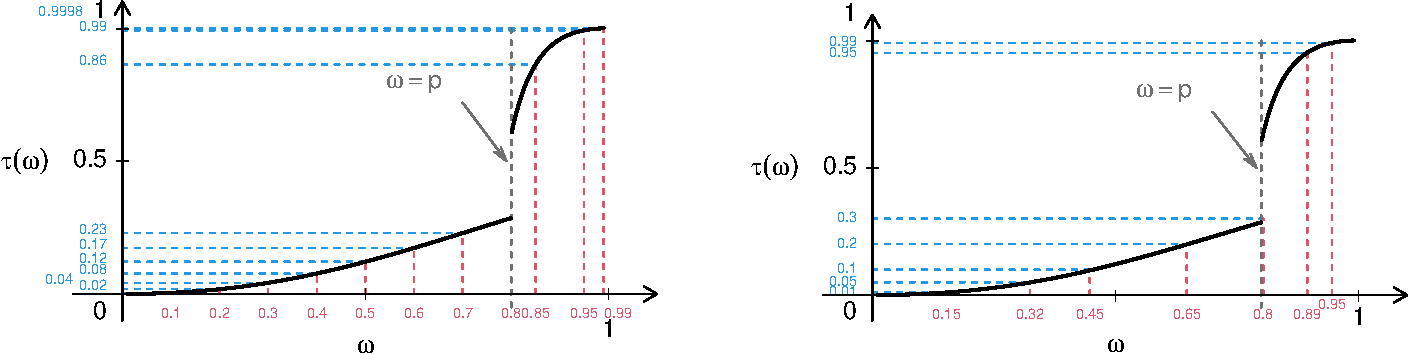
\includegraphics[width=0.8\linewidth]{traffic-expectiles_files/figure-latex/figcor-1} \caption{The quantile-expectile correspondence for the mixture of two uniform distributions in Example 3.4 for various quantile and expectile levels and $p=0.8$.}\label{fig:figcor}
\end{figure}

An estimate for the correspondence function can be obtained following the procedure of \citet{taylor2008}, who constructs the empirical cumulative distribution function by counting the observations below the estimated expectile for each of the \(\tau\)-levels, such that for each \(\tau\) there is a corresponding estimate of the quantile index \(\omega\). One can then interpolate linearly between the resulting points to obtain \(\hat\tau(\omega)\).

Therefore, any quantile is also an expectile via the quantile-expectile correspondence. Since expectiles are uniquely defined for any distribution with a finite mean and do not require invertibility of the cumulative distribution function, they are a well-defined alternative to quantiles. This is particularly beneficial for discrete travel time distributions, continuous mixtures with non-overlapping supports, or mixtures of discrete and continuous components.

\hypertarget{quantiles-and-expectiles-of-travel-time-distribution-as-maximizers-of-u_1dt-and-u_2dt}{%
\subsection{\texorpdfstring{Quantiles and expectiles of travel time distribution as maximizers of \(U_1(d,T)\) and \(U_2(d,T)\)}{Quantiles and expectiles of travel time distribution as maximizers of U\_1(d,T) and U\_2(d,T)}}\label{quantiles-and-expectiles-of-travel-time-distribution-as-maximizers-of-u_1dt-and-u_2dt}}

Now we come back to our traveler's utility function in the asymmetric linear and quadratic versions. The following proposition connects the optimal departure times to quantiles and expectiles of travel time distribution.

\begin{proposition}[Optimal departure time plans]
\protect\hypertarget{prp:proputil}{}\label{prp:proputil}Let \(U_a(d,T), a\in\{1,2\}\) specified in \eqref{eq:ua} be the traveler's utility function with \(0<\beta_a<\alpha_a<\gamma_a\) fixed. Let \(T\) be a random travel time with distribution function \(F\). Then, optimal departure time \(d_a^*\) corresponds to:

\begin{itemize}
\item
  the \(\tau_1\)-quantile \(q_{\tau_1}(T)\) of \(F\) in case of \(U_1(d,T)\),
\item
  the \(\tau_2\)-expectile \(e_{\tau_2}(T)\) of \(F\) in case of \(U_2(d,T)\),
\end{itemize}

with \(\tau_a=\frac{\gamma_a}{\gamma_a+\beta_a}\) and \(a\in\{1,2\}\). Alternatively, we can express the ratio \(\frac{\gamma_a}{\beta_a}\) in terms of \(\tau_a\) as \(\frac{\gamma_a}{\beta_a} = \frac{\tau_a}{1-\tau_a}.\)
\end{proposition}

\begin{proof}
Rewrite \(\mathbb EU_a(d,T)\) as:
\[\mathbb EU_a(d,T) = -\left[\alpha_a \mathbb E(T^a) + (\gamma_a+\beta_a)\mathbb E\left\{\frac{\beta_a}{\gamma_a+\beta_a}(d-T)^a\mathbf 1_{T<d}+ \frac{\gamma_a}{\gamma_a+\beta_a}(T-d)^a\mathbf 1_{T\geq d}\right\}\right].\]

Setting \(\tau_a=\frac{\gamma_a}{\gamma_a+\beta_a}\), we get:

\begin{align}
\mathbb EU_a(d,T) &= -\left[\alpha_a \mathbb E(T^a) + (\gamma_a+\beta_a)\mathbb E\left\{(1-\tau_a)(d-T)^a\mathbf 1_{T<d}+ \tau_a(T-d)^a\mathbf 1_{T\geq d}\right\}\right]\nonumber\\
&= -\left(\alpha_a \mathbb E(T^a) + (\gamma_a+\beta_a)\mathbb E\left[|T-d|^a\{(1-\tau_a)\mathbf 1_{T<d}+ \tau_a\mathbf 1_{T\geq d}\right\}\right)\nonumber\\
&= -\alpha_a \mathbb E(T^a) - (\gamma_a+\beta_a)\mathbb E||T-d||_{a,\tau_a}^a. \label{eq:as}
\end{align}
That is, maximizing \(\mathbb EU_a(d,T)\) over \(d\in\mathbb R\) is equivalent to minimizing \(\mathbb E||T-d||_{a,\tau_a}^a\) resulting in \(d_1^*=q_{\tau_1}(T)\) in case \(a=1\) and \(d_2^*=e_{\tau_2}(T)\) in case \(a=2\).
\end{proof}

Proposition \ref{prp:proputil} can be extended to a general setting with:
\begin{align}
\mathbb E U_p(d,T) = -\alpha_p \mathbb E(T) - (\gamma_p+\beta_p)\mathbb E||T-d||_{p,\tau}^p, 1\leq p <\infty\label{eq:up}
\end{align}
and thus incorporates asymmetric \(L_p\)-loss on the early and late delays.

The optimal departure time, \(d_p^*\), in this generalized setting corresponds to the so-called \(L_p\)-quantile introduced in \citet{chen96} as a result of minimizing \(\mathbb E||T-d||_{p,\tau_p}^p\) for \(0\leq\tau_p\leq 1\) and \(1\leq p <\infty\).

\(U_p(d,T)\) generalizes the classical asymmetric linear scheduling utility to a richer class of preference functions, where an additional parameter \(p\) can be used to adjust commuters' aversions to delays. In our further analysis, we focus on \(p\in \{1,2\}\) and the comparison of the resulting preferences.

\begin{center}\rule{0.5\linewidth}{0.5pt}\end{center}

Given the optimal choice (\(d_1^*= q_{\tau_1}(T)\) or \(d_2^*= e_{\tau_2}(T)\)), the second term in \eqref{eq:as} corresponds to the asymmetric version of the absolute deviation (\(a=1\)) and variance (\(a=2\)) of random travel times, respectively. As a result, we get the \(\tau\)-deviation and the \(\tau\)-variance of \(T\), denoted as \(Dev_\tau(T)\) and \(Var_\tau(T)\), respectively. The notions of \(Dev_\tau(T)\) and \(Var_\tau(T)\) were introduced in \citet{tran2019} and are defined as:

\begin{equation}
Dev_\tau(T) = \mathbb E ||T-q_{\tau_1}(T)||_{1,\tau_1} \label{eq:tdev}
\end{equation}

and
\begin{equation}
Var_\tau(T) = \mathbb E ||T-e_{\tau_2}(T)||^2_{2,\tau_2}. \label{eq:tvar}
\end{equation}

Furthermore, using the location scale invariance of quantiles in Proposition \ref{prp:propprops} for \(a=1\), we get the well-known result of \citet{fosgerau2010}, where the optimal departure time \(d_1^* = \mu + \sigma F^{-1}\left(\frac{\gamma_1}{\beta_1+\gamma_1}\right)\) with \(F\) being the cumulative distribution function of the standardized travel time. The result for \(a=2\) is new. Proposition \ref{prp:proputil} generalizes, therefore, the result of \citet{fosgerau2010} to \(a\in\{1,2\}\) and provides a unified understanding of how the considered type of utility function is linked to the distributional properties of travel time \(T\).

Note that, although unique quantiles can be defined using \eqref{eq:inf}, in utility terms commuters are \emph{indifferent} between departure time in the respective quantile value ranges. That is, the resulting departure time choice is still not well-defined for some levels \(\tau\). In the same time, the expectiles are uniquely defined for all \(\tau\in (0,1)\) for any distribution with finite mean. Moreover, since all expectiles depend on the whole distribution, they are all responsive to changes in distributional parameters as opposed to quantiles as shown in the examples above.

As mentioned previously, there exist the correspondence function between quantiles and expectiles of a given distribution, which maps each well-defined quantile \(q_{\alpha}(T)\) to an expectile \(e_{\tau(\alpha)}(T)\). Therefore, the expected utility maximization in \eqref{eq:eu2} produces the same choices for suitably chosen preference parameter \(\gamma/\beta\), as shown in proposition \ref{prp:proputil2} below. Moreover, the asymmetric quadratic preference class is richer than the asymmetric linear one, as it delivers well-defined solutions for every combination of scheduling preference parameters not only for distributions of \(T\) with strictly increasing \(F\) but also for discrete distributions or distribution with discontinuous support (see examples \ref{exm:ddqande} and \ref{exm:duqande}).

\begin{proposition}[Correspondence between $U_1$- and $U_2$-based choices]
\protect\hypertarget{prp:proputil2}{}\label{prp:proputil2}Let \(U_1(d,T)\) be the traveler's utility function with known \(\gamma_1>\beta_1>0\). Let \(T\) be a random travel time with distribution function \(F\) and a finite mean. Then, for each \(\tau_1 = \frac{\gamma_1}{\beta_1+\gamma_1}\), where \(F\) is invertible, there exist \(\tau_2\) and \(\gamma_2>\beta_2>0\) such that maximizing \(\mathbb E U_1(d,T)\) with respect to \(d\) is equivalent to maximizing \(\mathbb E U_2(d,T)\) with respect to \(d\), and thus both utilities produce the same choices in the expected utility sense.

\end{proposition}

\begin{proof}
Using Proposition \ref{prp:proputil}, the optimal departure plan \(d_1^*\) for \(U_1(d,T)\) satisfies:

\[d_1^* = \arg\min_{d\in \mathbb R^+}\mathbb E\left(||T-d||_{1,\tau_1}\right),\]

which corresponds to the \(\tau_1\)-quantile of \(T\) for \(\tau_1=\frac{\gamma_1}{\beta_1+\gamma_1}\). Wenn \(F\) is invertible in \(\tau_1\), there exist a map \(\tau_2\equiv\tau_2(\tau_1)\) such that for the \(\tau_2\)-expectile, \(e_{\tau_2}\), holds \(e_{\tau_2} = q_{\tau_1}\) (Propositon \ref{prp:corr}). That is:

\[d_1^* = \arg\min_{d\in \mathbb R^+}\mathbb E\left(||T-d||_{1,\tau_1}\right) = \arg\min_{d\in \mathbb R^+}\mathbb E\left(||T-d||_{2,\tau_2}^2\right) = d_2^*.\]

The parameters \(\gamma_2>\beta_2>0\) are related as:

\begin{equation}\frac{\gamma_2}{\beta_2+\gamma_2} = \tau_2(\tau_1) = \tau_2\left(\frac{\gamma_1}{\beta_1+\gamma_1}\right), \label{eq:tcor}
\end{equation}

or \(\frac{\gamma_2}{\beta_2} = \frac{\tau_2}{1-\tau_2},\) where \(\tau_2\equiv \tau_2\left(\frac{\gamma_1}{\beta_1+\gamma_1}\right)\) is the quantile-expectile correspondence relation.
\end{proof}

In summary, the considered scheduling utility functions share the property that the maximizers of the resulting expected utilities are the tail indices (the \(\tau\)-quantile or the \(\tau\)-expectile) of the random travel time, where the index \(\tau\) depends on the preference parameters (\(\tau=\gamma/(\beta+\gamma)\)). Moreover, via the quantile-expectile correspondence, a maximizer of \(\mathbb EU_2(d,t)\) is also a maximizer of \(\mathbb EU_1(d,t)\) for some suitable preference transformation \(\tilde\gamma/\tilde \beta\) obtained by the inversion of \eqref{eq:tcor} if the relevant \(\tau_1\)-quantile is unique. Hence, the choices induced by maximizing \eqref{eq:eu1} build a subset of the choices induced by \eqref{eq:eu2}, and the latter enables a richer preference representation.

\hypertarget{analysing-the-effects-of-availability-accessibility-and-extreme-travel-times-under-u_1td-and-u_2td}{%
\subsection{\texorpdfstring{Analysing the effects of availability, accessibility and extreme travel times under \(U_1(T,d)\) and \(U_2(T,d)\)}{Analysing the effects of availability, accessibility and extreme travel times under U\_1(T,d) and U\_2(T,d)}}\label{analysing-the-effects-of-availability-accessibility-and-extreme-travel-times-under-u_1td-and-u_2td}}

In Example \ref{exm:ddqande}, we used a two-value travel time distribution and discussed its applicability for modeling departure time choice in the context of a bike rental station, where a bike is available with probability \(p\). If there is an available bike, the total travel time is \(t_1\), otherwise a longer travel time, \(t_2\), must be taken into account.

In this section, we analyze the effects of increasing availability (by increasing \(p=\mathbb P(T=t_1)\)) and improving accessibility (by decreasing \(t_2\)). To derive the time-saving effects for the two preference types, we assume that \(\tau=\frac \gamma{\gamma+\beta}\) is uniformly distributed on a plausible interval \([p-\Delta,p+\Delta]\), where \(p=\mathbb P(T=t_1)\) and \(0<\Delta<\min(p,1-p)\).

\begin{enumerate}
\def\labelenumi{\arabic{enumi})}
\item
  \textbf{Time savings under \(U_1\) resulting from increasing the availability \(p\) on the interval \([p-\Delta,p+\Delta]\) from \(p_0\) to \(p_1\)}. Recall that in this example the optimal choices for preferences described by \(U_1\) are the quantiles:
  \[q_\tau = \begin{cases}t_1,&\tau\in[0,p]\\t_2,&\tau\in(p,1].\end{cases}\]
  The total time savings, \(tts_1\), resulting from changing \(p\) from \(p_0\) to \(p_1\) are:
  \[tts_1=(p_1-p_0)\cdot (t_2-t_1).\]
\item
  \textbf{Time savings under \(U_2\) resulting from increasing the availability \(p\) on the interval \([p-\Delta,p+\Delta]\) from \(p_0\) to \(p_1\)}.
  Recall that in this example the optimal choices for preferences described by \(U_1\) are the quantiles:
  \[e_\tau = \frac{(1-\tau)t_1p+ \tau t_2(1-p)}{(1-\tau)p + \tau(1-p)} = t_1\phi(1-\tau,p)+ t_2\phi(\tau,1-p),\]
  where \(\phi(x,y)=\frac{x y}{xy+(1-x)(1-y)}.\)
  The total time savings, \(tts_2\), resulting from changing \(p\) from \(p_0\) to \(p_1\) can be computed as:
  \[tts_2 = \frac 1{2\Delta}t_1\int_{p-\Delta}^{p+\Delta}\left(\phi(1-\tau,p_0)-\phi(1-\tau,p_1)\right)d\tau + t_2\int_{p-\Delta}^{p+\Delta}\left(\phi(\tau,1-p_0)-\phi(\tau,1-p_1)\right)d\tau.\]
\end{enumerate}

Likewise, the time savings effects can be calculated for the case of increasing accessibility in terms reducing the alternative travel time \(t_2\). The resulting time savings are illustrated as shaded areas in Figure \ref{fig:figex12}.

\begin{figure}
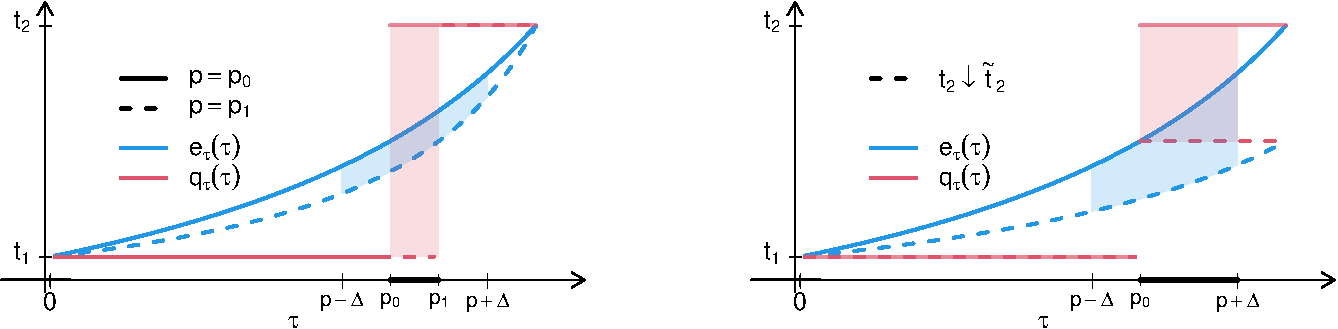
\includegraphics[width=1\linewidth]{traffic-expectiles_files/figure-latex/figex12-1} \caption{Left panel: the expectile and the quantile functions for the two-value discrete distribution with varying $p$. Right panel: the expectile and the quantile functions for the two-value discrete distribution with varying $t_2$}\label{fig:figex12}
\end{figure}

Although the absolute effect sizes (at least for our concrete choice of example values) in the quantile specification seem to dominate those in the expectile case, all commuters (\(\tau\in[p-\Delta,p+\Delta]\)) adjust their behavior in the expectile case. In contrast, for the quantile case, the change in \(p\) only influences commuters with preferences \(\tau\in[p_0,p_1]\) when \(p\) changes and \(\tau\in[p_0,p+\Delta]\) when \(t_2\) changes.

\begin{center}\rule{0.5\linewidth}{0.5pt}\end{center}

In Examples \ref{exm:duqande} and \ref{exm:qdzheng}, we considered mixtures of distributions to model travel times under two regimes: free flow and congestion. Let us now take a closer look at how commuters react to a higher probability of extreme travel times under both utility specifications.

\begin{figure}
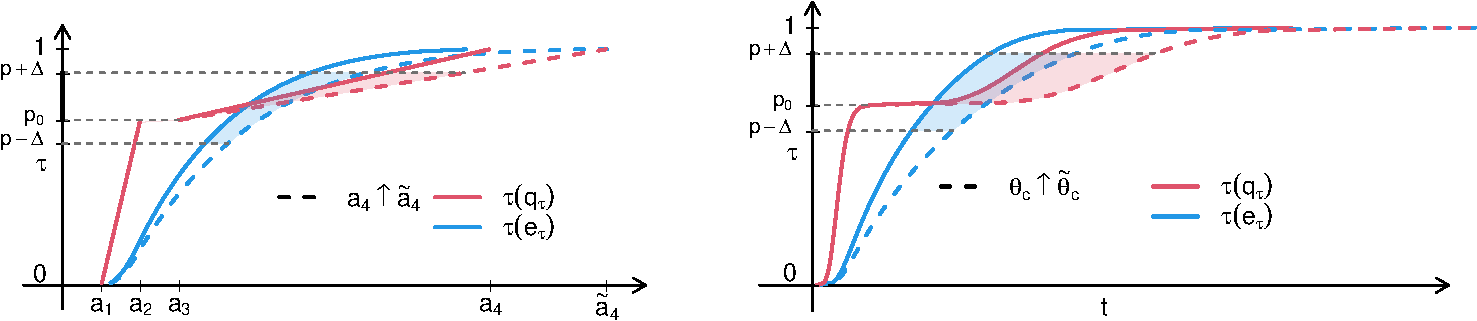
\includegraphics[width=1\linewidth]{traffic-expectiles_files/figure-latex/figexp22-1} \caption{Left panel: The inverse quantile and expectile functions for varying value of $a_4$ in Example 3.2. Right panel: The inverse quantile and expectile functions for varying value of the dispertion parameter $\theta_c$ in Example 3.3.}\label{fig:figexp22}
\end{figure}

On Figure \ref{fig:figexp22}, we observe departure time adjustments across the entire range of the preference parameter \(\tau\in[p-\Delta,p+\Delta]\) in the case of \(U_2\). In contrast, with \(U_1\), the behavioral reaction is limited to \(\tau\in[p_0,p+\Delta]\). From a behavioral perspective, it is not clear why only specific preference ranges are effected by the changes in travel time distribution.

Overall, \(U_2\) seem to capture preference adjustments to policy in a transparent and interpretable way, making it a valid alternative to the classical scheduling utility represented by \(U_1\).

\hypertarget{travel-time-reliability-ratio-under-asymmetric-scheduling-preferences}{%
\subsection{Travel time reliability ratio under asymmetric scheduling preferences}\label{travel-time-reliability-ratio-under-asymmetric-scheduling-preferences}}

As noted in \citet{li_etal17} and \citet{zang2022} among others, travel time reliability is a commonly recognized measure for assessing transportation network risks. Here we employ the Travel Time Reliability Ratio (TTRR), denoted here as \(\rho_a\), for quantifying travel time reliability in utility terms. This ratio relates the value of travel time variability and to the value of travel time, defined as (e.g., \citet{carrion_levinson12}):

\begin{align}
\rho_a = \frac{d\mathbb EU_a^*}{d\sigma^a_T}/\frac{d\mathbb EU_a^*}{d\mu_T}, \label{eq:rho}
\end{align}

where \(\mu_T\) and \(\sigma_T\) refer to the mean and the standard deviation of \(T\). Because the asymmetric quadratic
utility with \(a=2\) includes penalties for \emph{squared} early and late delays, it is reasonable to define the value of travel time variability in relation to \(\sigma_T^2\) to preserve unit consistency.

Assuming \(U_1\) is the traveler's utility function, \citet{fosgerau2010} show that the TTRR is:

\begin{align}
\rho_1 = \frac{d\mathbb EU_1^*}{d\sigma_T}/\frac{d\mathbb EU_1^*}{d\mu_T} = \frac{\beta+\gamma}{\alpha}\int_{\frac{\gamma}{\beta+\gamma}}^1 F^{-1}(p)dp.
\label{eq:rho11}
\end{align}

Computation of the right-hand-side of \eqref{eq:rho11} is not straightforward, and \citet{li2019} proposes a procedure based on the conditional value at risk to compute it. Below, we derive expressions for \(\rho_a, a\in\{1,2\}\) based on our notion of \(\mathbb EU_a(d,T)\), utilizing the expectation of an asymmetric norm. We propose computation based on empirical partial moments.

\begin{proposition}[Travel time reliability ratio]
\protect\hypertarget{prp:proprho}{}\label{prp:proprho}Let \(U_a(d,T), a\in\{1,2\}\) be the traveler's utility function as in \eqref{eq:ua} with \(\beta>0\) and \(\gamma>0\) known. Let \(T\) be a random travel time with distribution function \(F\) and a finite mean \(\mu_T\) and variance \(\sigma_T^2\). Then, the travel time reliability ratio \(\rho_a\) is determined as:

\[\rho_a = \frac{\gamma+\beta}{\alpha}\mathbb E||T_S-h_{a,\tau_a}(T_S)||_{a,\tau}^a,\]

where \(h_{a,\tau}(\cdot) = \begin{cases} q_\tau(\cdot),&\text{for } a=1,\\ e_\tau(\cdot),&\text{for }a=2,\end{cases}\) and \(\tau = \frac{\gamma}{\beta+\gamma}\).
\end{proposition}

\begin{proof}
Using \(h_{a,\tau}(T) = \sigma_T^a h_{a,\tau}(T_s)\) with \(T_S\) being the standardized version of \(T\) (Proposition \ref{prp:propprops}) and

\begin{align*}\mathbb E||T-h_{a,\tau}(T)||_{a,\tau}^a&=\mathbb E||(\sigma_TT_S + \mu_T)-(\sigma_Th_{a,\tau}(T_S)+\mu_T)||_{a,\tau}^a \\
&= \mathbb E||\sigma_T(T_S-h_{a,\tau}(T_S))||_{a,\tau}^a = \sigma_T^a\mathbb E||T_S-h_{a,\tau^*}(T_S)||_{a,\tau}^a,\end{align*}

we rewrite:

\[\mathbb E U_a^*(d,T) =-\alpha \mu_T - (\gamma+\beta)\mathbb E||T-h_{a,\tau}(T)||_{a,\tau}^a\\
=-\alpha \mu_T - (\gamma+\beta)\sigma_T^a\mathbb E||T_S-h_{a,\tau}(T_S)||_{a,\tau}^a.\]

The value of the travel time is:
\[\frac{d\mathbb EU_a^*}{d\mu_T} = -\alpha.\]
The value of the travel time variability is:
\[\frac{d\mathbb EU_a^*}{d\sigma^a_T} = -(\gamma+\beta)\mathbb E||T_S-h_{a,\tau}(T_S)||_{a,\tau}^a.\]
Plugging the above expressions in \eqref{eq:rho}, we get:
\[\rho_a=\frac{\gamma+\beta}{\alpha}\mathbb E||T_S-h_{a,\tau}(T_S)||_{a,\tau}^a.\]
\end{proof}

Proposition \ref{prp:proprho} shows, that for \(a=1\) we get:
\begin{equation}\rho_1 = \frac{(\gamma+\beta)}{\alpha}\mathbb E||T_S-q_{\tau_1}(T_S)||_{1,\tau_1}. \label{eq:rho1}
\end{equation}

In case \(a=2\), the TTRR becomes:
\begin{equation}\rho_2=\frac{\gamma+\beta}{\alpha}\mathbb E||T_S-e_{\tau_2}(T_S)||_{2,\tau_2}^2. \label{eq:rho2}
\end{equation}

The terms \(\mathbb E||T_S-q_{\tau_1}(T_S)||_{1,\tau_1}\) and \(\mathbb E||T_S-e_{\tau_2}(T_S)||_{2,\tau_2}^2\) represent respectively the \(\tau\)-deviation \(Dev_\tau(T_S)\) defined in \eqref{eq:tdev} and the \(\tau\)-variance \(Var_\tau(T_S)\) defined in \eqref{eq:tvar}. As discussed in the examples above, while \eqref{eq:rho1} can be problematic in situations where the respective quantiles are not well defined, an expectile-based measure in \eqref{eq:rho2} is feasible for all distributions with finite mean and variance.

The estimates for both expressions can be obtained using their empirical counterparts:

\begin{equation}\widehat{Dev_\tau} (T_S) = \frac 1n\sum_{i=1}^n |\tau^*- \mathbf 1_{t_{S,i}\leq q_{\tau^*}}|\cdot|t_{S,i}-\hat q_{\tau^*}|\label{eq:etdev}
\end{equation}
and

\begin{equation}\widehat{Var_\tau} (T_S) = \frac 1n\sum_{i=1}^n |\tau^*- \mathbf 1_{t_{S,i}\leq q_{\tau^*}}|\cdot |t_{S,i}-\hat q_{\tau^*}|^2\label{eq:etvar}
\end{equation}
which are both readily calculated from a sample of travel times. \citet{taylor2017} points out the importance of precise measurement of the right tail variation in order for such measure of variability to be useful for travelers in updating their behavior.

\begin{example}[TTRS for the distribution in Example 3.3]
\protect\hypertarget{exm:trrs}{}\label{exm:trrs}

In Examples \ref{exm:qdzheng}, we considered a mixture of two gamma distributions for travel time. Let us consider the TTRRs as functions of \(\tau=\frac{\gamma}{\gamma+\beta}\).

For larity, let us fix the utility parameters \(\alpha\) and \(\beta\), and rewrite the TTRR expressions using \(\gamma = \frac \tau{1-\tau}\cdot \beta\) as follows:

\begin{align}
\rho_a(\tau) &= \frac \beta\alpha\cdot\frac1{1-\tau}\cdot\mathbb E||T_S-q_{\tau_1}(T_S)||^a_{a,\tau_a}.
\end{align}

The evolution of the TTRR with \(\tau\) depends on the second part of the expression above, namely:

\[\xi_a(\tau)\equiv \frac1{1-\tau}\cdot\mathbb E||T_S-h_{a,\tau_a}(T_S)||_{a,\tau}^a,\]

which represents the \(\tau\)-deviation, \(Dev_\tau (T_s)\), for \(a=1\) and the \(\tau\)-variance, \(Var_\tau (T_S)\), for \(a=2\), respectively, weighted by \(\frac1{1-\tau}\). Neither \(Dev_\tau(T_S)\) nor \(Var_\tau(T_S)\) are monotonic in \(\tau\) in our mixture-of-gamma-distributions example, as shown on the left panel of Figure \ref{fig:figrho}. However, the weighted version, \(\xi_2(\tau)=\frac1{1-\tau}Var_\tau(T_S)\) is monotonic increasing in \(\tau\), whereas \(\xi_1(\tau)=\frac1{1-\tau}Dev_\tau (T_s)\) appears to have a small ``bump'' around the mixing parameter \(p\), caused by a low density region between the two modes of the mixed distribution. The resulting \(\rho_1(\tau)\) and \(\rho_2(\tau)\) for \(\tau\in[0.5,1)\) are shown the right panel of Figure \ref{fig:figrho}. The ``bump behavior'' of \(\rho_1(\tau)\) around \(p\) is undesirable from a utility perspective, since a small change in \(\tau\) (resulting from a small change in \(\gamma\)) could lead to a substantial \emph{decrease} in \(\rho_1(\tau)\) in the vicinity of \(p\). However, if the dense regions of mixing components overlap, the ``bump'' is smoothed out and the function becomes more even. In contrast, the TTRR resulting from our proposed asymmetric quadratic utility specification is a monotonic function of \(\tau\) and describes the reliability requirements of commuters in a more meaningful way.

\begin{figure}
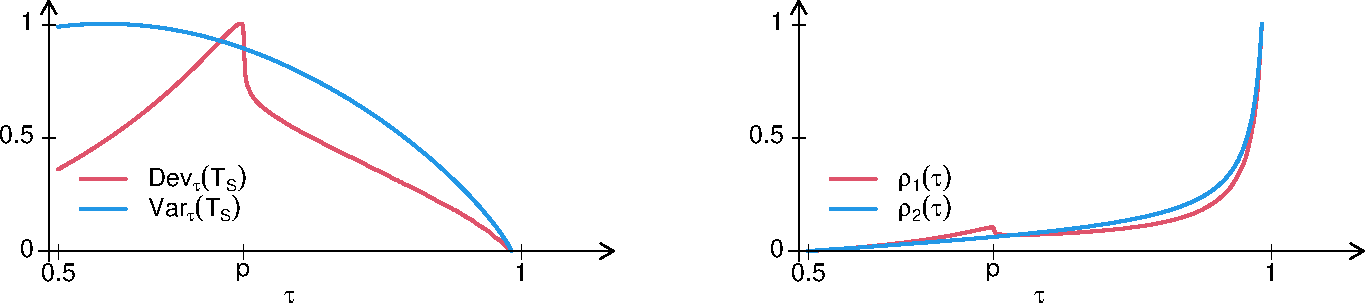
\includegraphics[width=1\linewidth]{traffic-expectiles_files/figure-latex/figrho-1} \caption{Left panel: $\tau$-deviation and $\tau$-variance as functions of $\tau$ scaled to the interval $[0,1]$. Right panel: TTRRs, $\rho_1(\tau)$ and $\rho_2(\tau)$, for the travel time distribution considerred in Example 3.3 (mixture of gamma distributions with mixing parameter $p$).}\label{fig:figrho}
\end{figure}

\end{example}

In summary, our framework for optimal departure time choices, represented as tail indices of the travel time distribution, establishes a connection between these optimal choices and the characteristics of the travel time distribution. This framework introduces a new type of scheduling utility function, with well-defined expected utility maximizers for various types of travel time distributions. Additionally, it simplifies the calculation of travel time reliability ratios induced by the considered utility types.

\hypertarget{empirical-validation-and-comparison-of-u_1td-and-u_2td}{%
\section{\texorpdfstring{Empirical validation and comparison of \(U_1(T,d)\) and \(U_2(T,d)\)}{Empirical validation and comparison of U\_1(T,d) and U\_2(T,d)}}\label{empirical-validation-and-comparison-of-u_1td-and-u_2td}}

In this section, we aim to empirically validate the proposed asymmetric quadratic utility specification using both an experimental dataset on route and departure time choices (Subsection 4.1) and observational travel time data from Montreal (Subsection 4.2).

\hypertarget{linear-and-squared-scheduling-losses-in-modelling-departure-time-choices}{%
\subsection{Linear and squared scheduling losses in modelling departure time choices}\label{linear-and-squared-scheduling-losses-in-modelling-departure-time-choices}}

To empirically validate the proposed utility specification, we compare two utility functions based on their scheduling loss components (linear vs.~quadratic) using a dataset from experiments on route and departure time choices (see \citet{Gonzalez2020} and \citet{GONZALEZRAMIREZ2021}), available at \url{https://figshare.com/articles/dataset/Experiments_on_route_and_departure_time/12388103} (accessed on 24.11.2024). The dataset includes computer-aided route choice experiments focused on diverse optimal departure time choices, involving a total of 496 participants and 5,535 recorded choices across 41 origin-destination pairs.

In these experiments, participants were asked to choose a route and a departure time for a given arrival time from a set of 5-minute departure slots. They were provided with information on route characteristics, travel time, as well as the maximum and minimum expected lateness for the available choices. This information on expected lateness---specifically, its average---serves as a useful proxy for the scheduling component of the considered utility functions. By analyzing choices based on the average of the maximum and minimum expected lateness for \(U_1\) and the average of their squared values for \(U_2\), we aim to assess which loss concept (linear versus quadratic) better captures realistic departure time choices.

We model the choices, labeled in the dataset as 1 (chosen) and 0 (rejected), using a binomial regression model with probit link, which is frequently used for binary choice modelling (\citet{ben1985discrete}). The explanatory variables include the travel time \(T\) provided in each experiment and either the average expected lateness (Model 1) or the average expected squared lateness (Model 2), denoted as \(ELATE\) and \(ELATE^2\), respectively. These variables are computed as follows:

\begin{align}ELATE &= \frac{ELATE\_max + ELATE\_min}2,\\
ELATE^2 &= \frac{ELATE^2\_max + ELATE^2\_min}2.
\end{align}
If \(ELATE\) is positive, we denote it as \(ELATE_{pos}\); otherwise, we write \(ELATE_{neg}\).

Since the participants were also provided with route characteristics, such as its length, directedness, number of turns and the percentage of freeway section on the route, which possibly influence the route choice, we also include those route characteristics as explanatory variables in the model (as columns of matrix \(R\) in the notation below).

Thus, our model specification representing the choices based on \(U_1\) (\(a=1\)) or on \(U_2\) (\(a=2\)) reads:

\begin{align}p(CHOICE=1|T_{i,j},ELATE^a_{pos,i,j}, ELATE^a_{neg,i,j}, R_j) = \Phi(\alpha_{1} T_{i,j} &+ \beta_{1} ELATE^a_{pos,i,j} + \gamma_1ELATE^a_{neg,i,j}\nonumber\\
&+ \delta_1R_{j,1},+ \ldots +\delta_4R_{j,4}) \label{eq:probit} \end{align}

where \(\Phi(z)\) denotes the distribution function of the standard normal distribution and \(p(CHOICE=1|T_{i,j},ELATE^a_{pos,i,j}, ELATE^a_{neg,i,j}, R_j)\) denotes the individual conditional probability of selecting time slot \(i\) on route \(j\) from the available time slots \(i=1, \ldots,n\), and routes \(j=1,\ldots,J\) based on the linear loss (\(a=1\)) or the squared loss (\(a=2\)) in the scheduling component.

To assess the goodness-of-fit of the models above, we employ a leave-one-out cross-validation procedure. First, we fit the models in \eqref{eq:probit} separately for each participant, using all but one route (containing a chosen departure time) for training. We then predict the participant's choice for the hold-out route based on the fitted models. The accuracy of these predictions is evaluated using the root mean squared prediction error (RMSPE) and the proportion of correctly predicted choices. A prediction is considered correct if the actual choice made by the participant corresponds to the time slot with the highest predicted probability. This cross-validation procedure is repeated until every route containing a chosen departure time has been left out once and the participant's choice has been predicted accordingly. The entire procedure---including fitting the probit choice models in \eqref{eq:probit} and performing cross-validation---is repeated for each participant.

\begin{table}
\centering
\caption{\label{tab:tableprobit}Cross-validation results on the model evaluation with linear (Model 1) and quadratic (Model 2) scheduling losses. The third specification (Model 1 or Model 2) indicates the case where one of the models is selected for each participant based on the in-sample residual deviance criterion.}
\centering
\begin{tabular}[t]{l|l|l|l|l}
\hline
Specification & Scheduling Loss & RMSPE & Prop. of correct predictions & Prop. of participants\\
\hline
Model 1 & linear & 0.1224 & 0.1537 & 0.2782\\
\hline
Model 2 & quadratic & 0.1221 & 0.1567 & 0.7218\\
\hline
Model 1 or Model 2 & linear or quadratic & 0.1220 & 0.1640 & 1.0000\\
\hline
\end{tabular}
\end{table}

\begin{table}
\centering
\caption{\label{tab:tabprobitres}Cross-validation results on the scheduling coefficient ratios for the linear (Model 1) and quadratic (Model 2) scheduling losses. $\overline{\hat \tau_{a,j}}$ corresponds to the mean, $\hat q_{0.5}({\hat \tau_{a,j} })$ - to the median, and $\hat q_{0.25}({\hat \tau_{a,j} })$ and $\hat q_{0.75}({\hat \tau_{k} })$ - to the lower and to the upper quartiles respectively.}
\centering
\begin{tabular}[t]{l|l|l|l|l|l}
\hline
Specification & Scheduling Loss & $\overline{\hat \tau_{a,j}}$ & $\hat q_{0.5}({\hat \tau_{a,j} })$ & $\hat q_{0.25}({\hat \tau_{a,j} })$ & $\hat q_{0.75}({\hat \tau_{k} })$\\
\hline
$a=1$ (Model 1) & linear & 0.7407 & 0.7676 & 0.5757 & 0.9888\\
\hline
$a=2$ (Model 2) & quadratic & 0.7664 & 0.8826 & 0.5726 & 0.9925\\
\hline
\end{tabular}
\end{table}

The results\footnote{All computations are performed in R (\citet{rr}). The probit regression is fitted using \emph{glm} function from the R-base. The associated code is available on \url{https://github.com/omanya/traffic-expectiles}}, aggregated across the participants, are presented in Table \ref{tab:tableprobit}. As seen in the table, while the root mean squared prediction errors of the two models are comparable, the proportion of correctly predicted choices is slightly higher when the quadratic loss specification is employed. Moreover, choosing the model specification for each participant based on the in-sample residual deviation, assigns Model 2 to a larger portion of decision makers (\(71.65\%\)) and achieves a large proportion of correct predictions. This suggests that the quadratic loss better captures actual departure time choices for a large portion of individuals in the experiment.

To further assess the model's plausibility and the preference distribution among participants, we report the average (\(\overline{\hat \tau_{a,j} }\)), the median (\(q_{0.5}({\hat \tau_{a,j} })\)), the lower quartile (\(q_{0.25}({\hat \tau_{a,j} })\)), and the upper quartile (\(q_{0.75}({\hat \tau_{a,j} })\)) for the scheduling coefficient ratios, defined as:
\[\hat \tau_{a,j} = \frac{\hat\gamma_{a,j}}{\hat\beta_{a,j}+\hat\gamma_{a,j}}\]
in Table \ref{tab:tabprobitres}. Here, \(\hat\alpha_{a,j}\), \(\hat\beta_{a,j}\), and \(\hat\gamma_{a,j}\) denote the estimated coefficients of the \(a\)-th model, with \(a=1\) for the asymmetric linear and \(a=2\) for the asymmetric quadratic losses, and \(j=1,\ldots,J\) representing the participant index. The resulting coefficient ratios appear plausible. The majority of participants seem to be highly averse to late arrivals, as the distribution of preferences \(\{\hat\tau_{a,j}\}_{j=1}^J\) tends to favor high values with a relatively high probability for both model specifications.

Overall, these results suggest that the quadratic loss specification provides a more accurate representation of departure time choices compared to the linear loss model for a large portion of decision makers. The strong aversion to late arrivals observed across the participants further supports the relevance of incorporating a squared scheduling loss in utility-based departure time models.

\hypertarget{optimal-departure-time-choices-under-u_1td-and-u_2td-for-montreal-travel-time-data}{%
\subsection{\texorpdfstring{Optimal departure time choices under \(U_1(T,d)\) and \(U_2(T,d)\) for Montreal travel time data}{Optimal departure time choices under U\_1(T,d) and U\_2(T,d) for Montreal travel time data}}\label{optimal-departure-time-choices-under-u_1td-and-u_2td-for-montreal-travel-time-data}}

In this section, we provide a real data example, considering a non-trivial travel time distribution, using the dataset of travel times for Montreal (the data is available at
{[}https://donnees.montreal.ca/dataset/temps-de-parcours-sur-des-segments-routiers-historique{]} (https://donnees.montreal.ca/dataset/temps-de-parcours-sur-des-segments-routiers-historique) and was accessed on 21 Aug 2024). We take two subsets of trips from 2019 on links LND\_1E-1B and LSh\_01-40, collected between 6:00 and 8:00 am on regular working days (Monday through Thursday). The two links are considered as alternative routes in the analysis. As indicated by the kernel density estimates in the left panel of Figure \ref{fig:choices}, the data appear to be generated by a model with several regimes. Following \citet{jabari2019}, we model the data using a \(k\)-component mixture of gamma distributions. The number of components, \(k=2\), for both subsets was selected based on the Akaike Information Criterion.

All computations are performed in R (\citet{rr}). The mixture of gamma distributions is fitted using the \emph{mixtools} package (\citet{mixtools}). The empirical counterparts of quantiles and expectiles are computed utilizing the \emph{quantile} function from the R-base and the \emph{expectile} function from the \emph{expectreg} package (\citet{expectregl}, \citet{expectreg}).

\begin{table}

\caption{\label{tab:tabpars}The estimated parameters of the two-component gamma mixture model (sample sizes $n_{1}=13992$ and $n_{2}=1166$).}
\centering
\begin{tabular}[t]{l|l|l|l|l|l|l|l|l|l|l}
\hline
  & $p_{1,.}$ & $k_{1,.}$ & $\theta_{1,.}$ & $p_{2,.}$ & $k_{2,.}$ & $\theta_{2,.}$ & $\mu_{1,.}$ & $\mu_{2,.}$ & $\sigma_{1,.}$ & $\sigma_{2,.}$\\
\hline
route 1 & 0.46 & 21.69 & 0.30 & 0.54 & 9.77 & 1.28 & 6.51 & 12.55 & 1.40 & 4.01\\
\hline
route 2 & 0.49 & 32.58 & 0.25 & 0.51 & 6.54 & 2.11 & 8.14 & 13.78 & 1.43 & 5.39\\
\hline
\end{tabular}
\end{table}

As shown in Table \ref{tab:tabpars}, the estimated models for route 1 and route 2 travel times assign similar probabilities for the free-flow regime, captured by the first component (0.46 and 0.49 respectively), and the congestion regime (0.54 and 0.51 respectively). Note that, although the second model is associated with a higher probability of the free-flow regime (0.49 compared to 0.46), it also reveals higher means and standard deviations in both regimes (\(\mu_{1,2}=8.14\) and \(\mu_{1,2}=13.78\) compared to \(\mu_{1,1}=6.51\) and \(\mu_{1,2}=12.55\), as well as \(\sigma_{1,2}=1.43\) and \(\sigma_{1,2}=5.39\) compared to \(\sigma_{1,1}=1.4\) and \(\sigma_{1,2}=4.01\)), resulting in higher probability of right extremes. In the following analysis, we examine the choices based on the proposed utility formulations.

The corresponding optimal departure time choices for both utility types are plotted in Figure \ref{fig:choices}. On the right panel of the figure, we show the estimated optimal choices as quantiles for \(U_1\) and expectiles for \(U_2\), varying the preference parameter \(\tau=\frac{\gamma}{\beta+\gamma}\). We estimate the quantiles and the expectiles based on the fitted mixture distributions using Monte-Carlo approximation and the formulas in \eqref{eq:q} and \eqref{eq:e}.

\begin{figure}
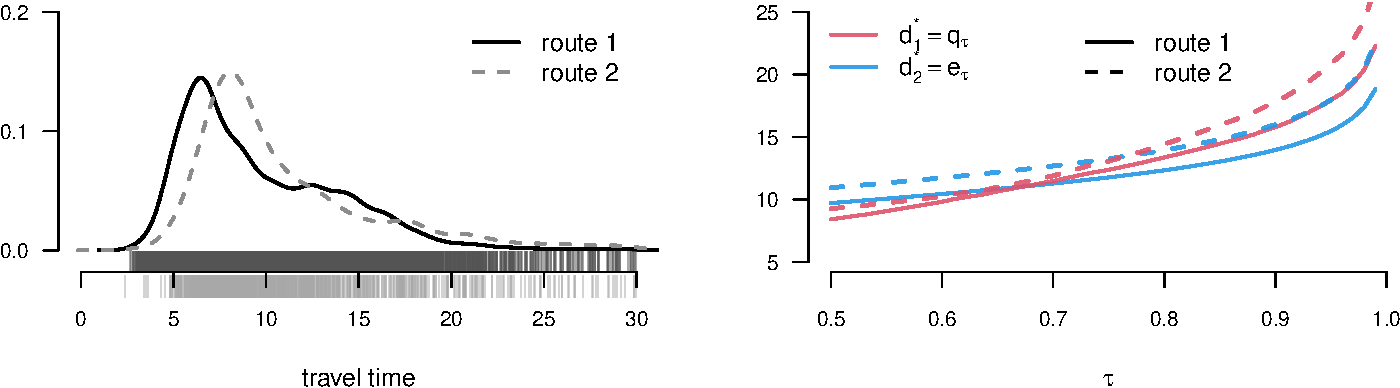
\includegraphics[width=1\linewidth]{traffic-expectiles_files/figure-latex/choices-1} \caption{Left panel: Kernel density estimates for the considered travel times. Right panel: Optimal choices as the quantiles for $U_1$ and expectiles for $U_2$  under different preference specification $\tau$ based on the fitted mixture model.}\label{fig:choices}
\end{figure}

As shown in Figure \ref{fig:choices}, the optimal departure times under \(U_1\) are slightly below the optimal departure times under \(U_2\) for lower \(\tau\)-values. For the \(\tau\)-values between \(0.6\) and \(0.7\), the quantile departure times are nearly the same for both routes. For higher \(\tau\)-values, the quantile departure time choices increasingly reflect the right tail of the distribution, leading to a greater divergence between the routes. In contrast, the evolution of the expectile choices remains even, as it takes both the probabilities and magnitudes into account.

For this example, we also estimate the quantile-expectile correspondences \(\tau_2(\tau_1)\) for \(\tau_1\in(0.5,1)\), as shown in the left plot of Figure \ref{fig:figcor2} for both routes, to directly compare the resulting TTRRs. The TTRR curves as functions of \(\tau\) are obtained using \eqref{eq:etdev} and \eqref{eq:etvar} and are illustrated in the right panel of Figure \ref{fig:figcor2}. The \(\rho_2\)-values on the figure are adjusted using the estimated correspondences \(\hat\tau_2(\tau_1)\) and \eqref{eq:tcor}. The TTRR curves associated with \(U_1\) cross at \(\tau=0.65\), indicating mixed preferences. The TTRRs associated with \(U_2\) for route 2 are consistently higher than those for route 1 at the same \(\tau\), reflecting its greater exposure to extreme travel times.

\begin{figure}
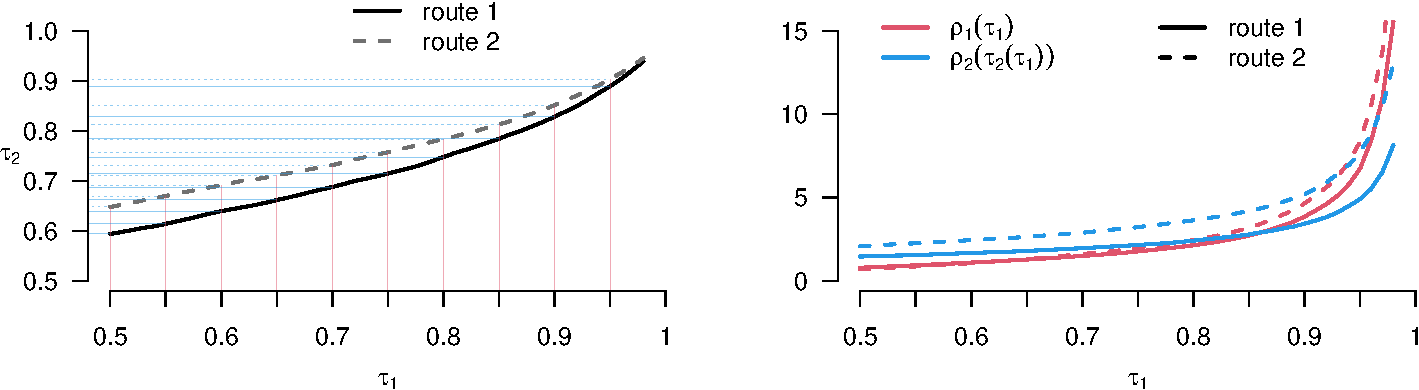
\includegraphics[width=1\linewidth]{traffic-expectiles_files/figure-latex/figcor2-1} \caption{Left panel: Quantile-expectile correspondences for the considerred travel time data. Right panel: TTRRs for both utility specifications for the considerred travel time data and utility parameters $\beta=1$, $\alpha=2\beta$, and $\gamma = \beta\tau/(1-\tau)$ for the $\tau_2$-values matched on the $\tau_1$-values through the estimated quantile-expectile correspondence.}\label{fig:figcor2}
\end{figure}

Overall, in the application above, we used a mixture of gamma distributions to model travel times and obtained optimal departure time choices for \(U_1(d,T)\) and \(U_2(d,T)\) across various preference combinations. The application demonstrates the advantages of our new expectile-based utility specification, which delivers more plausible departure time choices in line with the risk profile of each route to all preference specifications. Additionally, the TTRR values based on \(U_2\) and computed via the sample \(\tau\)-variance clearly reflect the higher risk exposure of route 2 compared to route 1, unlike the TTRRs derived from \(U_1\). This provides potential advantages for modeling risk perception in transportation networks in general and for individual route choice considerations in particular.

\hypertarget{conclusion}{%
\section{Conclusion}\label{conclusion}}

In this paper, we examine two specifications of scheduling utility: the classical asymmetric linear function of early and late delays and a new specification based on the asymmetric quadratic loss. Our framework connects the resulting optimal departure time choices, represented as tail indices of the travel time distribution, with the characteristics of the travel time distribution. This framework introduces a new type of scheduling utility function, which allows for well-defined expected utility maximizers across various travel time distributions and simplifies the calculation of travel time reliability ratios induced by the considered utility types.

Specifically, we show that the optimal departure choices for both utilities are the tail indices of the travel time distribution and can be analysed as the maximizers of expectations in suitably defined asymmetric norms. For the asymmetric linear specification, those are the quantiles, while for the asymmetric quadratic specification, they are the expectiles. Since expectiles are unique for any distribution with a finite mean, our new asymmetric quadratic specification does not rely on the assumption of an invertible cumulative distribution function. The induced optimal choices are unique for discrete travel time distributions, mixtures of components with non-overlapping supports, and mixtures with discrete and continuous components as in \citet{zheng_fangfang2017} and \citet{depalma2006}. Moreover, expectiles are more sensitive than quantiles to changes in the tail regions of the travel time distribution, which is valuable for capturing commuters' sensitivity to extremes as observed by \citet{enide2006}, \citet{vanlint_etal08}, and \citet{sikka_hanley13}.

Additionally, we derive the travel time reliability ratios for both utility types using our expection-in-an-asymmetric-norm approach. We show, that the resulting travel time reliability ratios of the asymmetric quadratic utility specification more clearly reflect the risk profiles of travel time distribution. Moreover, in our formulation, these reliability ratios can be easily estimated using the concepts of the \(\tau\)-deviation and the \(\tau\)-variance from \citet{tran2019}, via straightforward calculations of their empirical counterparts.

Using a dataset on departure time choices, we test both scheduling loss specifications, finding that the quadratic loss specification more accurately represents actual departure time choices. The strong aversion to late arrivals observed across participants further supports the relevance of our proposed asymmetric quadratic utility specification.

Finally, we apply our approach to travel time data from Montreal, fitting a mixture of gamma components to empirically examine how optimal departure choices evolve with varying preference parameters under both utility specifications. We estimate the quantile-expectile correspondence, compare the resulting travel time reliability ratios, and highlight the advantages of the asymmetric quadratic utility specification, positioning it as a viable alternative to the classical scheduling utility. This approach offers potential benefits for modeling various risk perceptions in transportation networks.

\hypertarget{declaration-of-generative-ai-and-ai-assisted-technologies-in-the-writing-process}{%
\section*{Declaration of generative AI and AI-assisted technologies in the writing process}\label{declaration-of-generative-ai-and-ai-assisted-technologies-in-the-writing-process}}
\addcontentsline{toc}{section}{Declaration of generative AI and AI-assisted technologies in the writing process}

Statement: During the preparation of this work the author used ChatGPT in order to improve the readability and language of the manuscript. After using this tool/service, the author reviewed and edited the content as needed and takes full responsibility for the content of the published article.

\bibliography{traffic-expectiles.bib}


\end{document}
